\chapter{One-factor Hull-White Model}

\section{Tests of implementation...}

The Monte-Carlo simulation is based on the pseudo short rate $x(t)$ defined by
\begin{equation}
x(t) = r(t) - f(0,t),
\end{equation}
where $x(0) = 0$.

The corresponding pseudo discount function is given by
\begin{equation}
X(t) = \exp \left( - \int_0^t x(u) du \right)
\end{equation}
hence, the real discount function is given by
\begin{equation}
D(t) = \exp \left( - \int_0^t r(u) du \right) = P(0,t) \exp \left( - \int_0^t x(u) du \right) = P(0,t) X(t).
\end{equation}


\begin{figure}
\centering
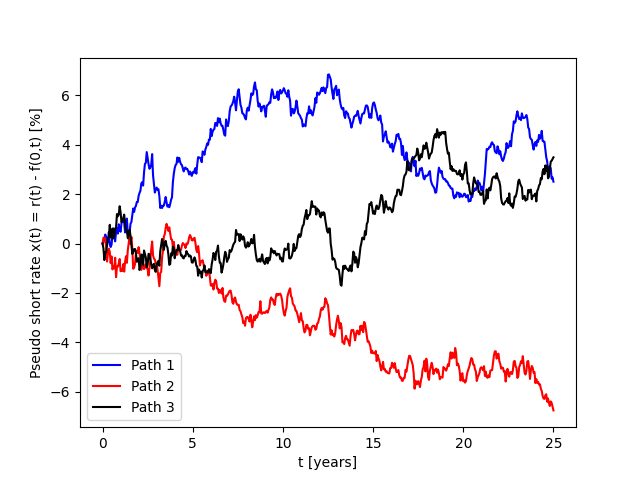
\includegraphics[scale=0.7]{figures/pseudo_short_rate_paths.png}
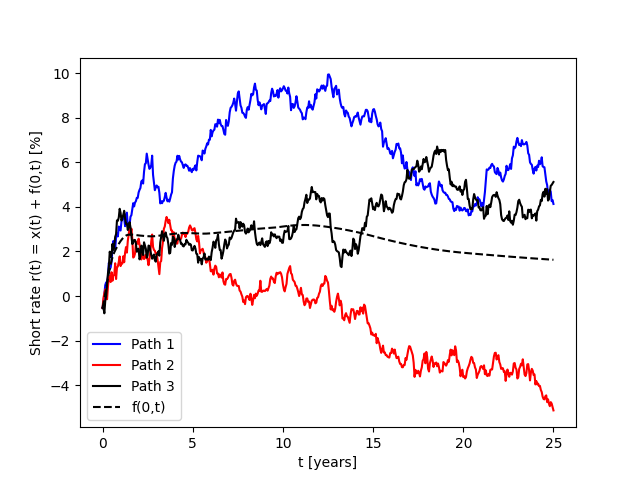
\includegraphics[scale=0.7]{figures/short_rate_paths.png}
\caption{Monte-Carlo paths for $x(t)$ and $r(t)$...}
\end{figure}

\begin{figure}
\centering
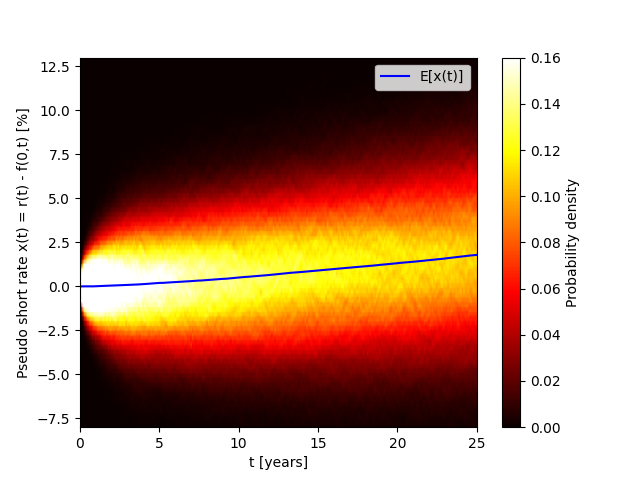
\includegraphics[scale=0.7]{figures/pseudo_short_rate_density.png}
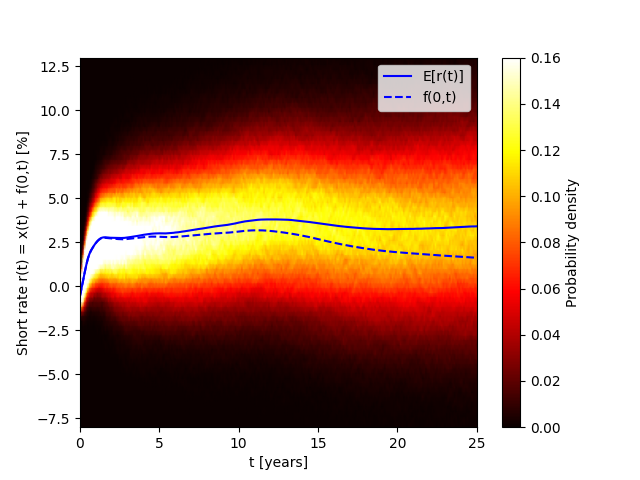
\includegraphics[scale=0.7]{figures/short_rate_density.png}
\caption{Density plots of $x(t)$ and $r(t)$...}
\end{figure}

\begin{figure}
\centering
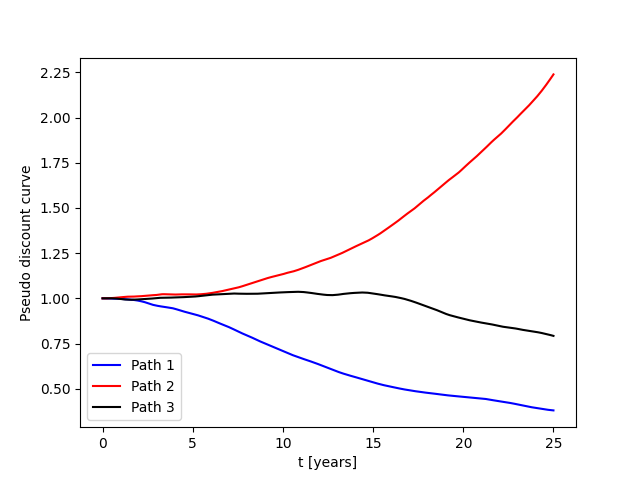
\includegraphics[scale=0.7]{figures/pseudo_discount_paths.png}
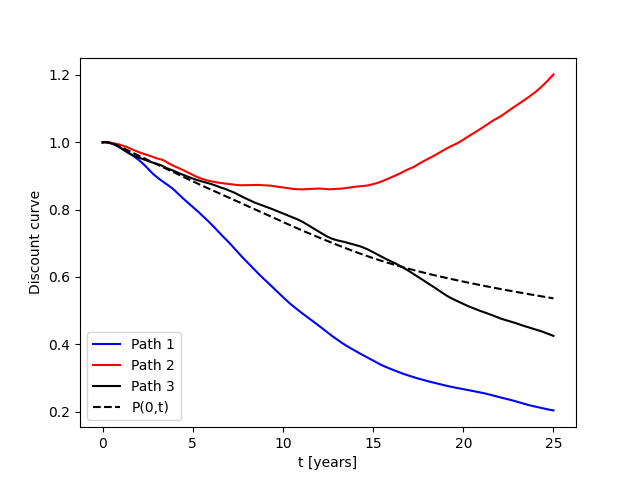
\includegraphics[scale=0.7]{figures/discount_paths.png}
\caption{Monte-Carlo paths for $X(t)$ and $D(t)$...}
\end{figure}

\begin{figure}
\centering
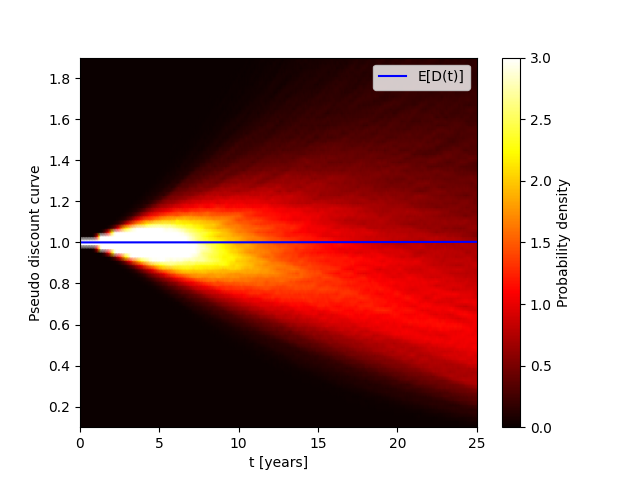
\includegraphics[scale=0.7]{figures/pseudo_discount_density.png}
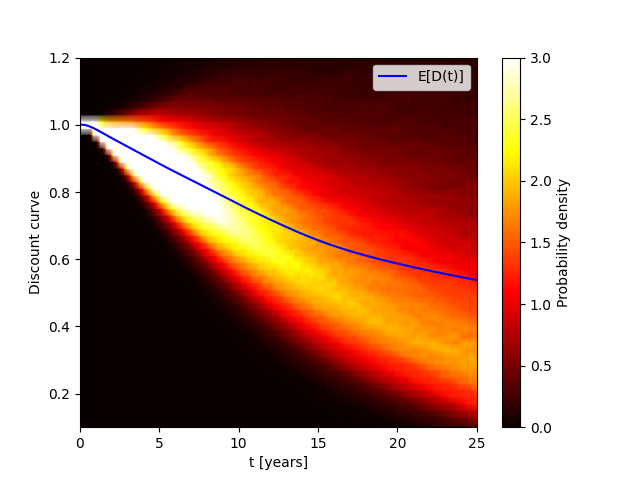
\includegraphics[scale=0.7]{figures/discount_density.png}
\caption{Density plots of $X(t)$ and $D(t)$...}
\end{figure}

\section{Tests of Monte-Carlo convergence}
